\documentclass{beamer}
%
% Choose how your presentation looks.
%
% For more themes, color themes and font themes, see:
% http://deic.uab.es/~iblanes/beamer_gallery/index_by_theme.html
%
\mode<presentation>
{
  \usetheme{default}      % or try Darmstadt, Madrid, Warsaw, ...
  \usecolortheme{wolverine} % or try albatross, beaver, crane, ...
  \usefonttheme{default}  % or try serif, structurebold, ...
  \setbeamertemplate{navigation symbols}{}
  \setbeamertemplate{caption}[numbered]
} 

\usepackage[spanish]{babel}
\usepackage[utf8x]{inputenc}
\usepackage{subcaption}

\title[Toma de decisión en juegos de azar]{Reconocimiento de manos ganadoras en el truco}
\author{Nahuel Lascano \newline Pablo Somodi \newline Agostina Villanueva}
\institute{Departamento de Computación - FCEyN - UBA}
\date{3 de noviembre de 2014}

\begin{document}

\begin{frame}
  \titlepage
\end{frame}

% Uncomment these lines for an automatically generated outline.
%\begin{frame}{Outline}
%  \tableofcontents
%\end{frame}

\section{Experimento}

\begin{frame}{Objetivos}

\begin{itemize}
  \item Entender cómo es el algoritmo usado para reonocer al ganador en una mano de Truco.
  \item Detectar situaciones que complican o facilitan esta decisión.
\end{itemize}

\end{frame}


\begin{frame}{Motivación}

\begin{itemize}
\item Queríamos estudiar la toma de decisiones en juegos de azar.
\item El Truco es el juego de cartas por excelencia en muchos países de Latinoamérica.
\item Hay pocos estudios al respecto.
\end{itemize}

\end{frame}

\begin{frame}{El experimento}
\begin{itemize}

\item Se le presentan al sujeto de prueba cartas enfrentadas y se le pide que indique el ganador lo más rápido posible.
\pause
\item Primera parte:
  \begin{itemize}
  \item Mostramos ``rondas'': dos cartas enfrentadas.
  \item 2 tandas de 25 rondas cada una.
  \end{itemize}
\item Segunda parte:
  \begin{itemize}
  \item Mostramos manos completas: 6 cartas enfrentadas de a pares.
  \item 4 tandas de 25 manos cada una.
  \end{itemize}
\pause
\item Entre las rondas/manos presentadas hay algunas aleatorias y otras armadas específicamente para testear lo que queremos.
  \begin{itemize}
  \item La primera tanda de cada parte siempre era con cartas aleatorias.
  \end{itemize}
\item Después de cada respuesta mostrábamos si había sido correcta o no.
\item Hicimos la prueba con 34 sujetos.
\item Registramos correctitud y tiempo de respuesta para cada ronda/mano mostrada.
\end{itemize}
\end{frame}


\begin{frame}{El análisis - Primera parte}
\begin{itemize}
\item Para cada sujeto, comparamos cada grupo de rondas contra un ``grupo control'' con un \textit{paired student's t-test}.
\item Descartamos los tiempos en los que el sujeto respondía incorrectamente.
\item El grupo control consistía en pares de cartas con un ganador claro que no cumplieran las características de los demás grupos.
\end{itemize}
\end{frame}

\begin{frame}{La gente aprende}
\begin{figure}
   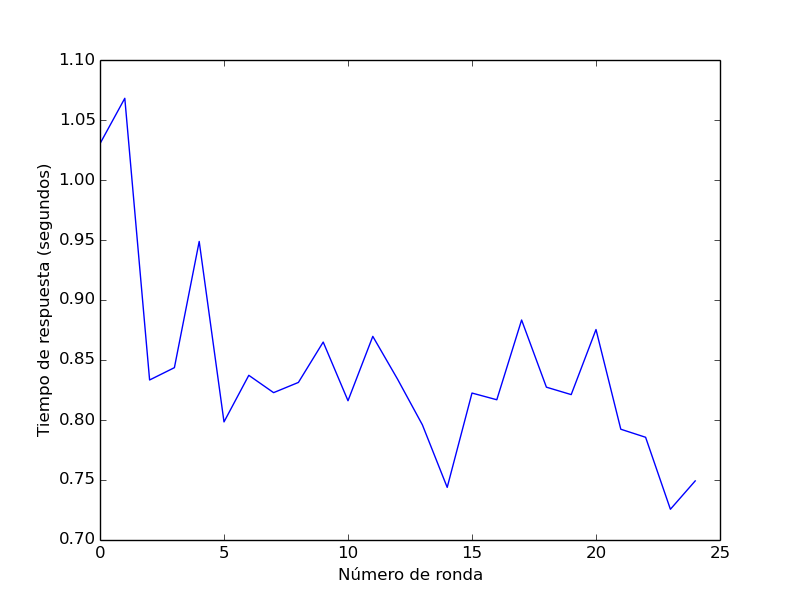
\includegraphics[width=0.8\linewidth]{graficos/tiempo_por_ronda.png}
\end{figure}
\begin{center}A raíz de esto, para todos los tests posteriores tiramos los primeros 3 datos.
\end{center}
\end{frame}


\begin{frame}{Ancho de espada}
\begin{figure}
   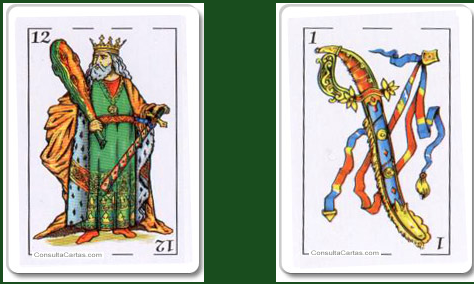
\includegraphics[width=0.8\linewidth]{examples_img/rondas_1.png}
\end{figure}
\begin{center}¿Será significativo?
\pause
\textbf{¡Muy!\ }($p \approx 1.953*10^{-6}$)
\end{center}
\end{frame}

\begin{frame}{Ancho de espada}
\begin{figure}
   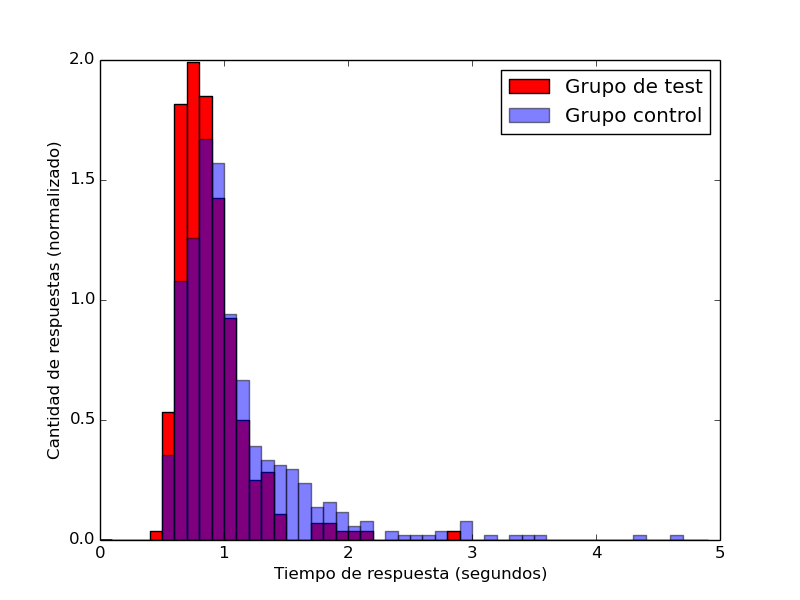
\includegraphics[width=0.9\linewidth]{graficos/rondas1vs5.png}
\end{figure}
\begin{center}
$p \approx 1.95*10^{-6}$
\end{center}
\end{frame}

\begin{frame}{Cartas buenas}
\begin{figure}
   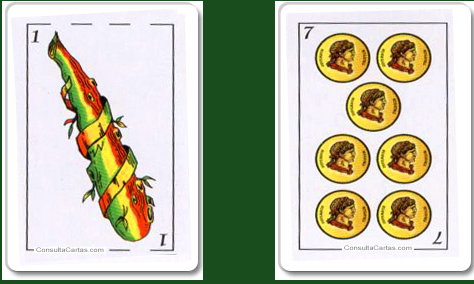
\includegraphics[width=0.8\linewidth]{examples_img/rondas_2.png}
\end{figure}
\begin{center}¿Será significativo?
\pause
\textbf{No\ }($p \approx 0.76758$)
\end{center}
\end{frame}

\begin{frame}{Figuras}
\begin{figure}
   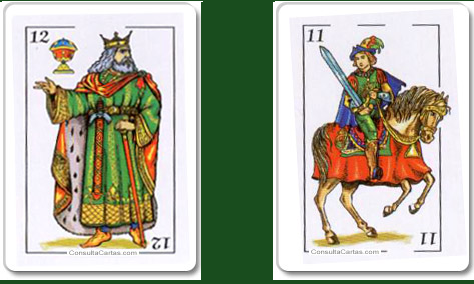
\includegraphics[width=0.8\linewidth]{examples_img/rondas_3.png}
\end{figure}
\begin{center}¿Será significativo?
\pause
Sí, la gente responde \textbf{más rápido.\ }($p \approx 0.00045$)
\end{center}
\end{frame}

\begin{frame}{Figuras}
\begin{figure}
   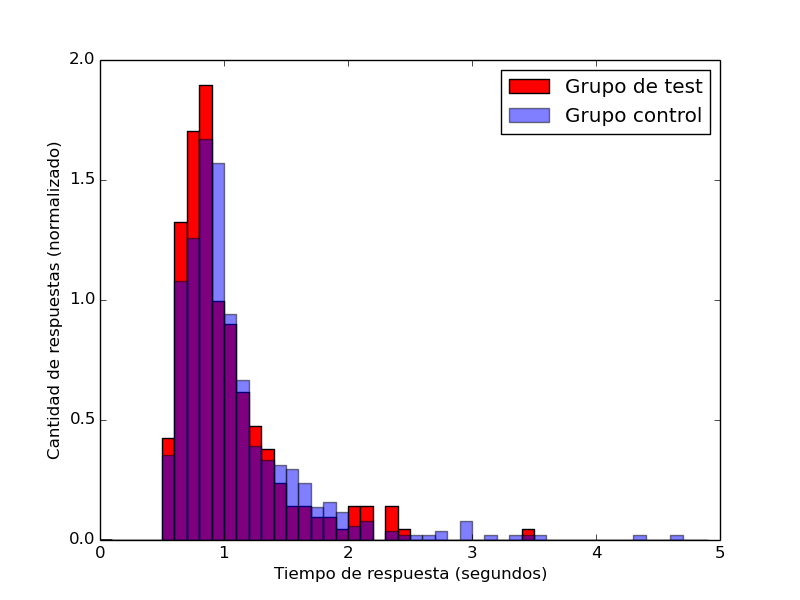
\includegraphics[width=0.9\linewidth]{graficos/rondas3vs5.png}
\end{figure}
\begin{center}$p \approx 0.00045$
\end{center}
\end{frame}

\begin{frame}{Cartas malas}
\begin{figure}
   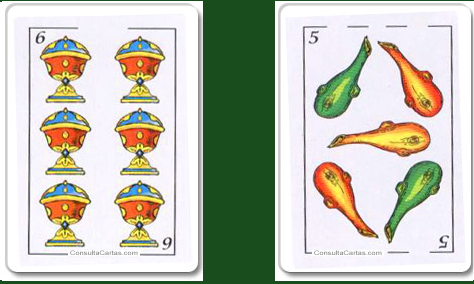
\includegraphics[width=0.8\linewidth]{examples_img/rondas_4.png}
\end{figure}
\begin{center}¿Será significativo?
\pause
Sí, la gente responde \textbf{más lento\ }($p \approx 0.00248$)
\end{center}
\end{frame}

\begin{frame}{Cartas malas}
\begin{figure}
   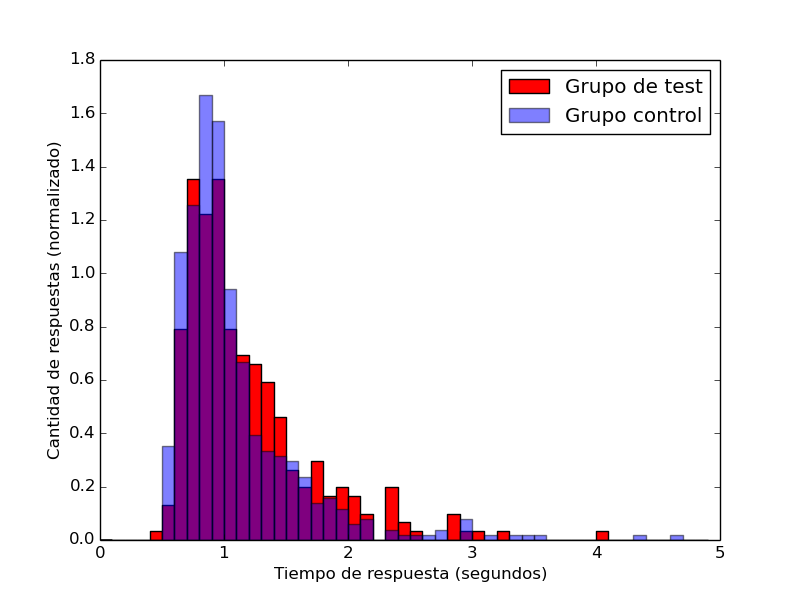
\includegraphics[width=0.9\linewidth]{graficos/rondas4vs5.png}
\end{figure}
\begin{center}$p \approx 0.00248$
\end{center}
\end{frame}

\begin{frame}{Anchos falsos}
\begin{figure}
   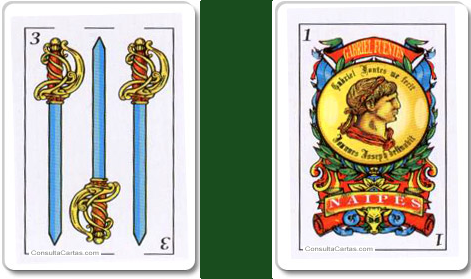
\includegraphics[width=0.8\linewidth]{examples_img/rondas_6.png}
\end{figure}
\begin{center}¿Será significativo?
\pause
\textbf{No\ }($p \approx 0.37008$)
\end{center}
\end{frame}

\begin{frame}{Sietes falsos}
\begin{figure}
   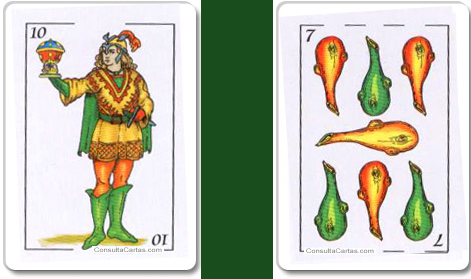
\includegraphics[width=0.8\linewidth]{examples_img/rondas_7.png}
\end{figure}
\begin{center}¿Será significativo?
\pause
\textbf{No\ }($p \approx 0.3894$)
\end{center}
\end{frame}

\begin{frame}{El análisis - Segunda parte}
\begin{itemize}
\item De nuevo comparamos, para cada sujeto, cada grupo de manos contra un ``grupo control'' con un \textit{paired student's t-test}.
\item Descartamos los tiempos en los que el sujeto respondía incorrectamente.
\item El grupo control consistía en 3 rondas, cada una de ellas con un ganador claro, y se definía en la 3ra ronda.
\end{itemize}
\end{frame}

\begin{frame}{Nuevamente la gente aprende}
\begin{figure}
   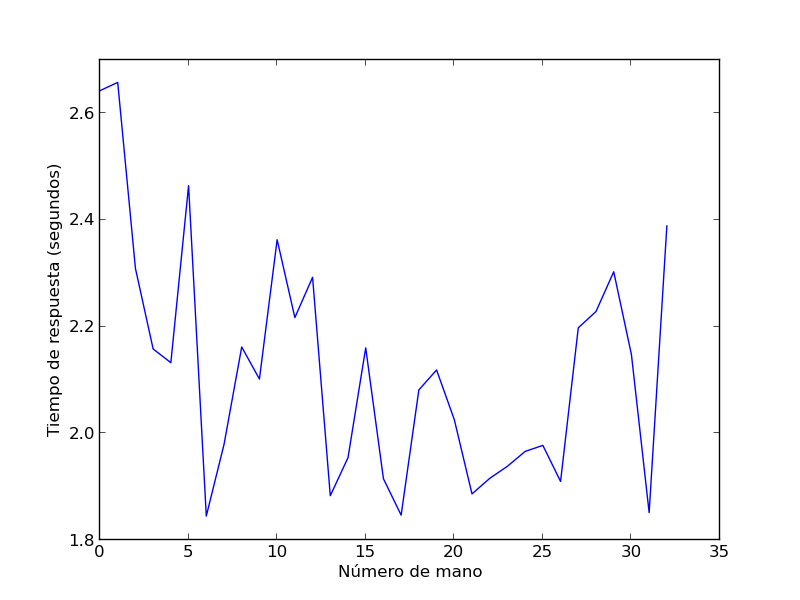
\includegraphics[width=0.8\linewidth]{graficos/tiempo_por_mano.png}
\end{figure}
\begin{center}De nuevo tiramos los primeros 3 datos.
\end{center}
\end{frame}


\begin{frame}{El algoritmo UCR}
\begin{itemize}
\item Una forma sencilla de decidir quién gana en una mano es mirar quién gana la última ronda.
\item Llamamos a este algoritmo UCR ("Últimas Cartas Reveladas")
\item Si incluímos a los que usan UCR nos rompe el análisis de tiempos.
\pause

\begin{figure}
	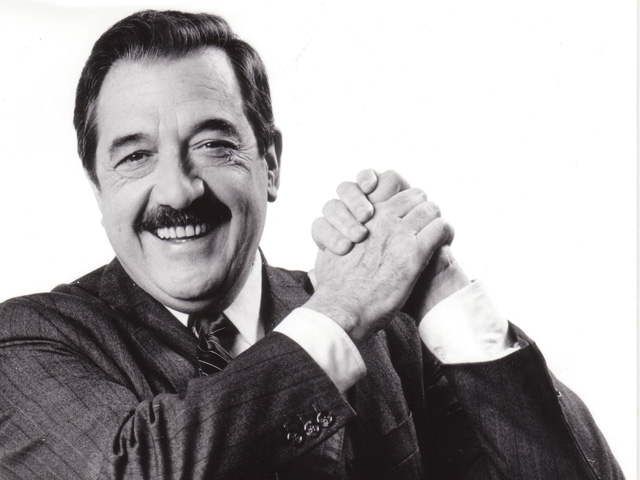
\includegraphics[width=0.7\linewidth]{alfonsin.jpg}
\end{figure}

\end{itemize}
\end{frame}


\begin{frame}{El algoritmo UCR}
  \begin{columns}
    \begin{column}{.4\linewidth}
	  	\begin{itemize}
        \item Para filtrarlos, les pusimos trampas.
        \item Consideramos que alguien usó UCR si falló más del 50\% de las manos trampa.
        \item Un 21\% de los sujetos de prueba lo usaba.
        \end{itemize}
    \end{column}
    \begin{column}{.6\linewidth}
     \begin{figure}
        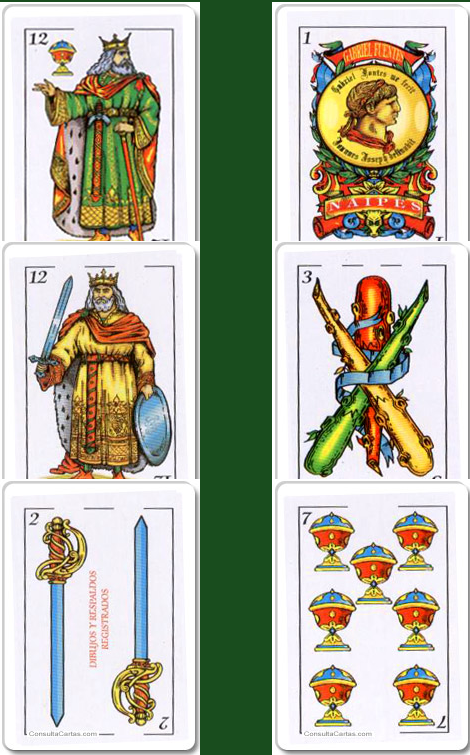
\includegraphics[width=0.75\linewidth]{examples_img/manos_1.png}
     \end{figure}
    \end{column}
  \end{columns}
\end{frame}

\begin{frame}{2 pares}
  \begin{figure}
  	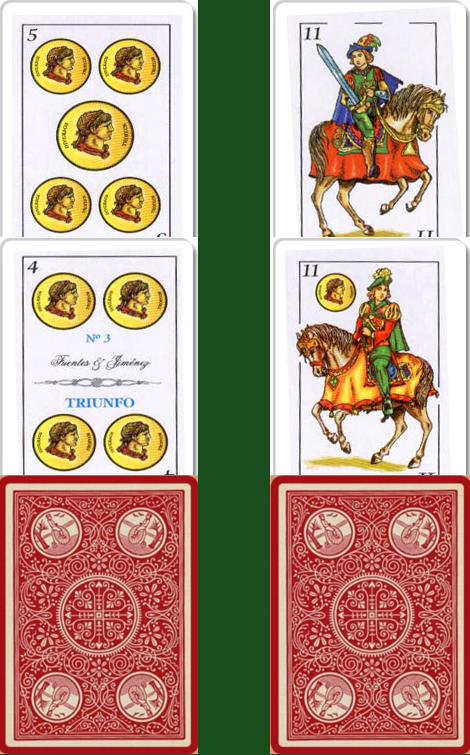
\includegraphics[width=0.4\linewidth]{examples_img/manos_2.png}
  \end{figure}
  \begin{center}
  ¿Será significativo?
  \pause
  \textbf{¡Efectivamente!} ($p \approx 2.79967*10^{-10}$)
  \end{center}
\end{frame}

\begin{frame}{2 pares}
  \begin{figure}
  	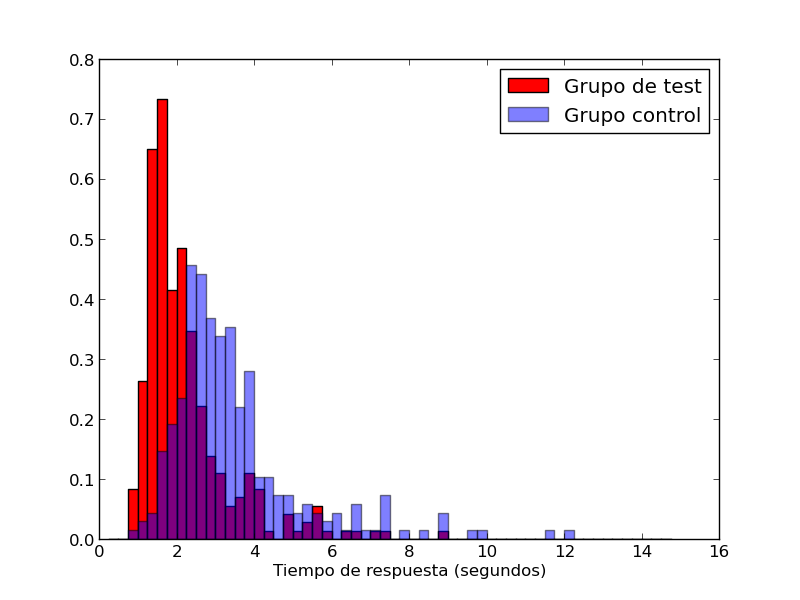
\includegraphics[width=0.8\linewidth]{graficos/2vs3.png}
  \end{figure}
  
  \begin{center}$p \approx 2.79967*10^{-10}$
  \end{center}
\end{frame}

\begin{frame}{Parda en 1ra y 2da}
  \begin{figure}
  	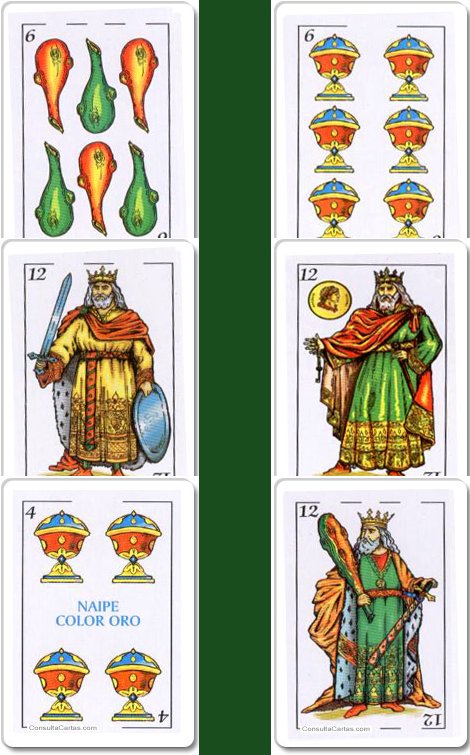
\includegraphics[width=0.4\linewidth]{examples_img/manos_4.png}
  \end{figure}
  \begin{center}
  ¿Será significativo?
  \pause
  \textbf{No} ($p \approx 0.34206$)
  \end{center}
\end{frame}

\begin{frame}{Parda en 3ra}
  \begin{figure}
  	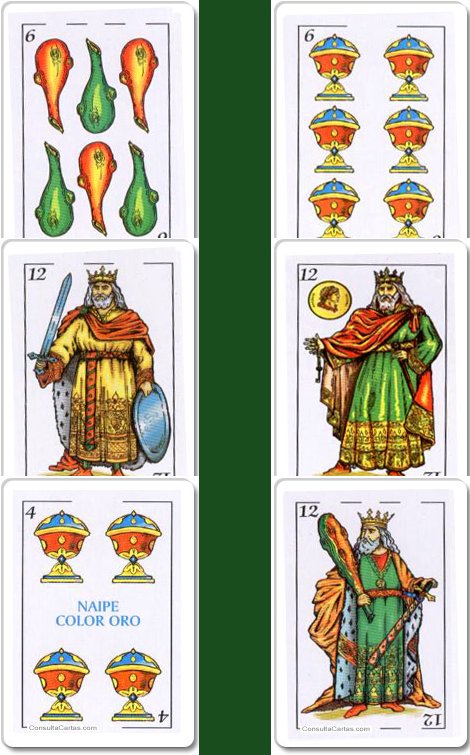
\includegraphics[width=0.4\linewidth]{examples_img/manos_4.png}
  \end{figure}
  \begin{center}
  ¿Será significativo?
  \pause
  Sí, la gente responde \textbf{más lento} ($p \approx 0.00681$)
  \end{center}
\end{frame}

\begin{frame}{Parda en 3ra}
  \begin{figure}
  	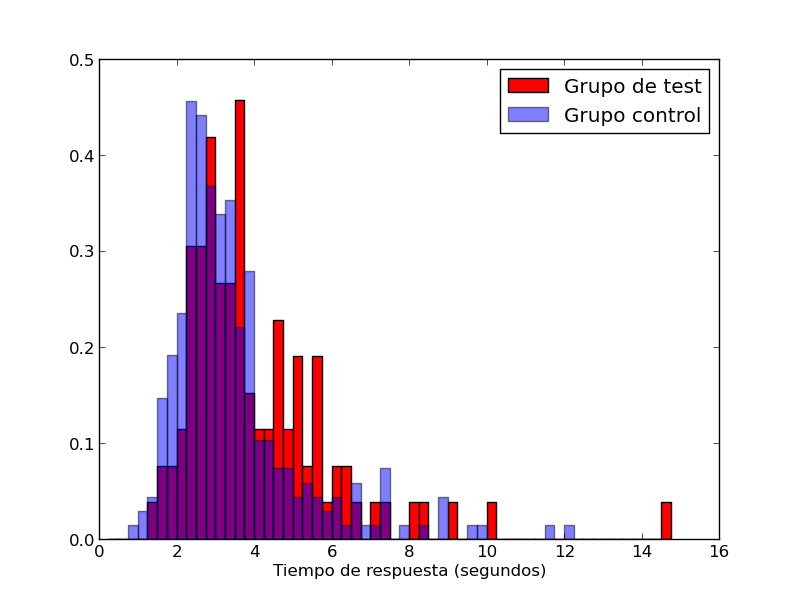
\includegraphics[width=0.8\linewidth]{graficos/5vs3.png}
  \end{figure}
  \begin{center}$p \approx 0.00681$
  \end{center}
\end{frame}

\begin{frame}{Parda en todas}
  \begin{figure}
  	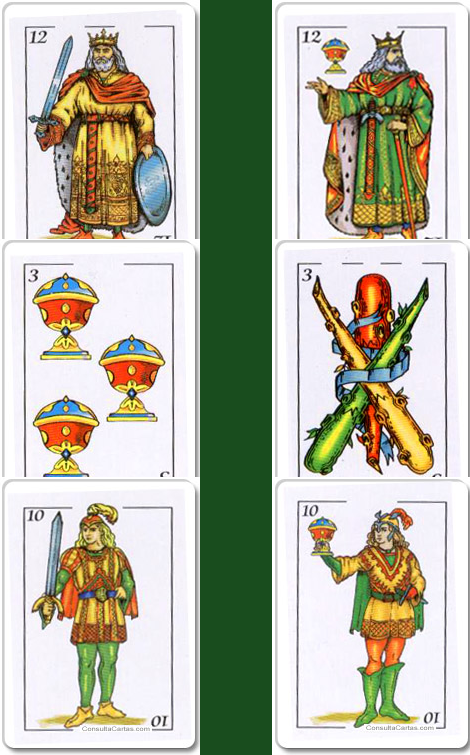
\includegraphics[width=0.4\linewidth]{examples_img/manos_6.png}
  \end{figure}
  \begin{center}
  ¿Será significativo?
  \pause
  \textbf{No} ($p \approx 0.21056$)
  \end{center}
\end{frame}

\begin{frame}{Figuras}
  \begin{figure}
  	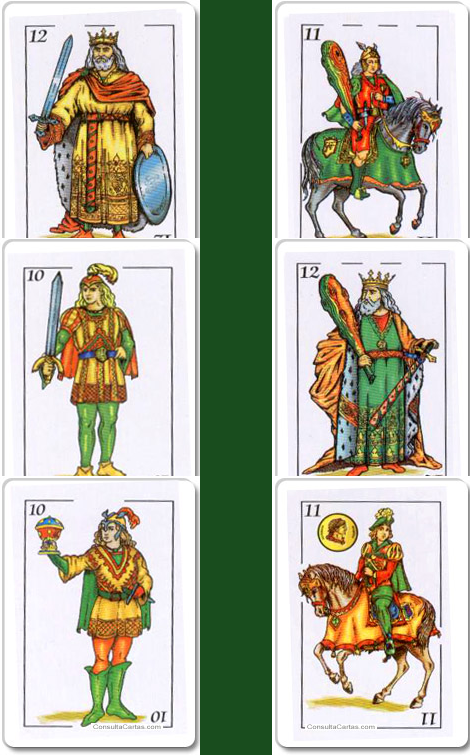
\includegraphics[width=0.4\linewidth]{examples_img/manos_7.png}
  \end{figure}
  \begin{center}
  ¿Será significativo?
  \pause
  \textbf{No} ($p \approx 0.14642$)
  \end{center}
\end{frame}

\begin{frame}{Carta fuerte del lado perdedor}
  \begin{figure}
  	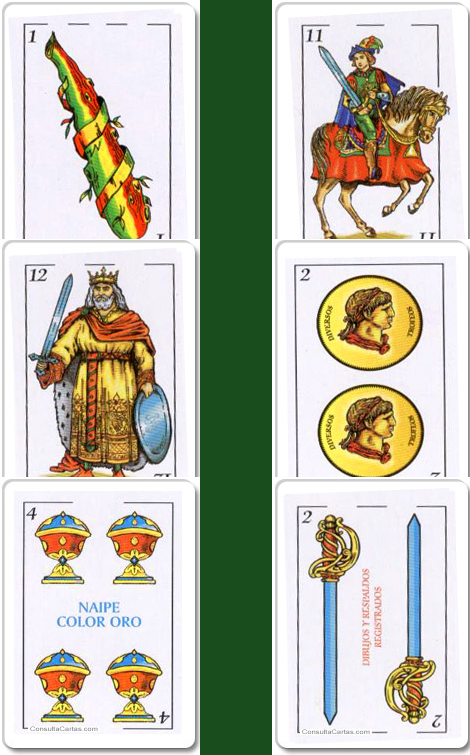
\includegraphics[width=0.4\linewidth]{examples_img/manos_10.png}
  \end{figure}
  \begin{center}
  ¿Será significativo?
  \pause
  Sí, la gente responde \textbf{más lento} ($p \approx 0.00173$)
  \end{center}
\end{frame}

\begin{frame}{Carta fuerte del lado perdedor}
  \begin{figure}
  	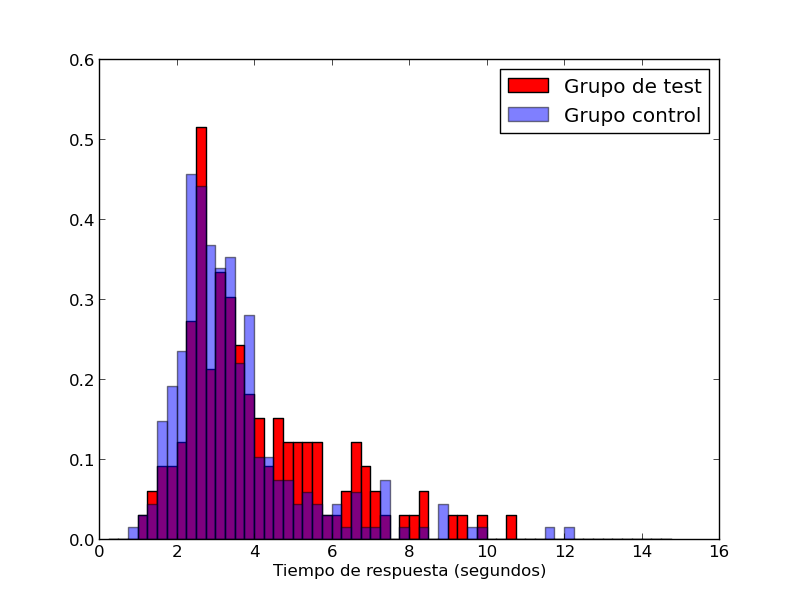
\includegraphics[width=0.8\linewidth]{graficos/10vs3.png}
  \end{figure}
  \begin{center}$p \approx 0.00173$
  \end{center}
\end{frame}

\begin{frame}{Usuarios de UCR}
Por otro lado, los que clasificamos como usuarios de UCR:
\begin{itemize}
\item No se ven afectados por cartas fuertes del lado perdedor ni responden más rápido cuando solo hay 2 rondas.
\item Pero sí responden significativamente más lento cuando hay parda en la 3ra o pardas en todas las rondas.
\end{itemize}
\end{frame}

\begin{frame}{Usuarios de UCR}
    \begin{columns}[c] % the "c" option specifies center vertical alignment
    \column{.5\textwidth} % column designated by a command
    	\begin{figure}
        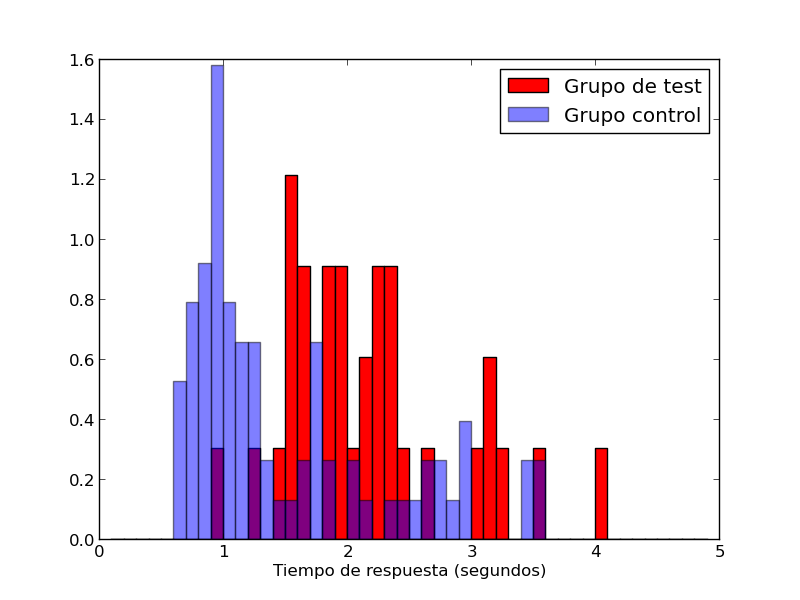
\includegraphics[width=1\linewidth]{graficos/5vs3ucr.png}
    	\caption{Manos con parda en la 3ra $(p \approx 0.00367)$}
        \end{figure}
    \column{.5\textwidth}
    	\begin{figure}
        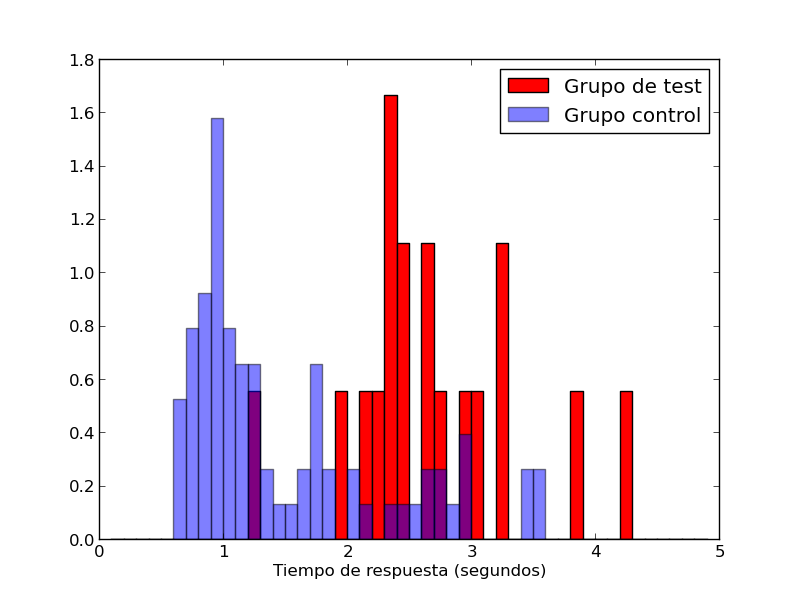
\includegraphics[width=1\linewidth]{graficos/6vs3ucr.png}
    	\caption{Manos con parda en todas $(p \approx 0.00307)$}
    	\end{figure}   
    \end{columns}
\end{frame}


\begin{frame}{El algoritmo}
\begin{itemize}
\item Muchas cosas nos llevan a pensar que la gente analiza la mano ronda por ronda de principio a fin.
\item Para verificarlo, graficamos el promedio de tiempos para todos los sujetos (que no usan UCR):
	\begin{itemize}
    \item para las rondas sueltas
    \item para las manos de dos rondas
    \item para las manos de tres rondas "simples"
    \item para las manos de tres rondas con parda en la 3ra
    \end{itemize}
\end{itemize}
\end{frame}

\begin{frame}{El algoritmo: regresión lineal}
\begin{figure}
  	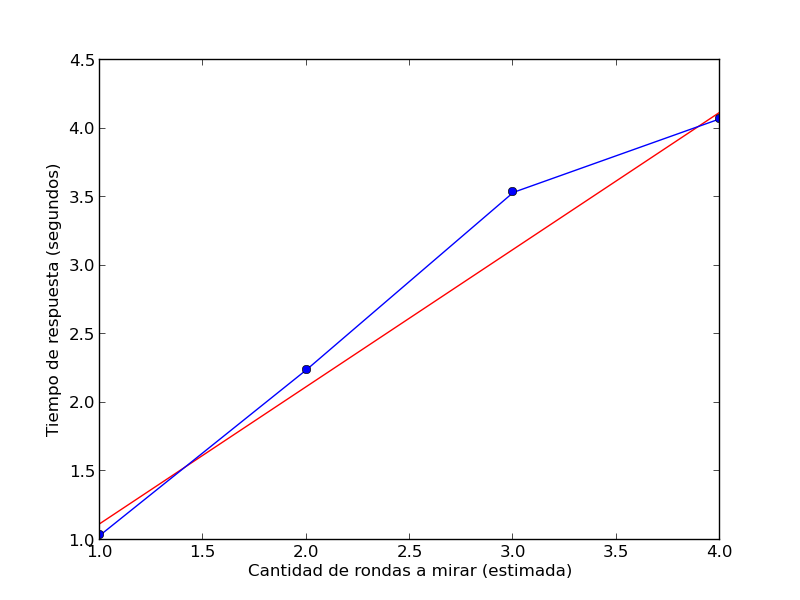
\includegraphics[width=0.7\linewidth]{graficos/lineal.png}
  \end{figure}
Pendiente: 			1.04022, 
Ordenada al origen: 0.12013 \\
R-Value: 			0.98661,  
P-Value:			0.01339 \\
Error estándar: 	0.12161
\end{frame}

\begin{frame}{Algunas conclusiones}
\begin{itemize}
\item Es mucho más rápido decidir quién gana una ronda si el ancho de espada aparece en ella.
\item Es más lento decidirlo cuando se enfrentan dos cartas muy malas.
\item La gente tiene bien incorporado el valor de los sietes falsos y anchos falsos.
\pause
\item Es más difícil determinar que alguien perdió cuando tiene una carta fuerte (7 de oro para arriba).
\item Para decidir el ganador de una mano, parecería que la gente mira linealmente las rondas de arriba hacia abajo, pero sin recordar quién ganó primera.
\begin{itemize}
	\item Por eso una parda en primera y segunda no hacen la decisión más difícil,
    \item Pero una parda en la tercera sí.
\end{itemize}
\pause
\item Muchas cosas que pensamos que podían ser significativas no lo eran.
\end{itemize}
\end{frame}

\begin{frame}{Más conclusiones}
\begin{itemize}
\item Un 20\% de las personas siguen mirando solo la última ronda incluso cuando se le dió feedback negativo al respecto repetidas veces.
\item El resto dejó de hacerlo al recibir feedback negativo, o ni se avivó de que servía hacerlo.
\end{itemize}
\end{frame}


\begin{frame}{Ideas futuras}
Algunas ideas que no llegamos a desarrollar:
\begin{itemize}
  \item Comprobar los casos en los que la gente usa UCR hasta recibir feedback negativo en una mano tramposa.
  \item Comprobar si la gente demora más inmediatamente después de un error.
  \item Comprobar qué tipo de manos producen más errores.
  \item Ver específicamente qué cartas altas del lado perdedor hacen que cueste más determinar al ganador.
\end{itemize}
\end{frame}

\begin{frame}{Yapa}
\begin{itemize}
  \item El $C_{2}H_{6}O$ empeora significativamente la velocidad de respuesta pero no modifica los algoritmos usados.
\end{itemize}
\pause
\begin{figure}
	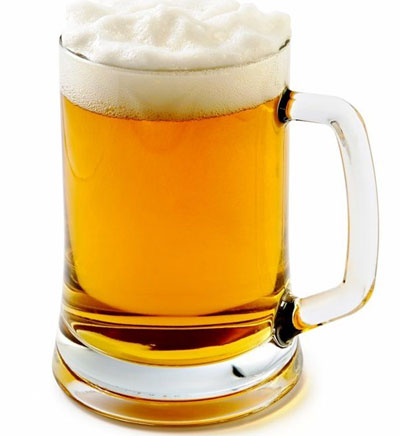
\includegraphics[width=0.6\linewidth]{birra.jpg}
\end{figure}
\end{frame}


\begin{frame}{Fin}
\begin{center}
\huge{\textbf{¡Gracias!}}
\end{center}
\end{frame}
\end{document}
